\section{Implementação Serial}

\begin{frame}{Java Serial --- Como Funciona}
    \begin{itemize}
        \item A cada iteração, o algoritmo \alert{relê o CSV do disco} inteiro
        \item Para cada linha: converte texto para números, calcula o cluster mais próximo, acumula
        \item Tudo em uma única thread --- leitura e computação misturados
    \end{itemize}

    \vspace{0.8em}
    \begin{block}{Expectativa}
        O gargalo deveria ser a aritmética do K-Means --- é ela que é executada milhões de vezes.
    \end{block}
\end{frame}

\begin{frame}{Onde o Tempo é Gasto? (JFR)}
    \begin{center}
        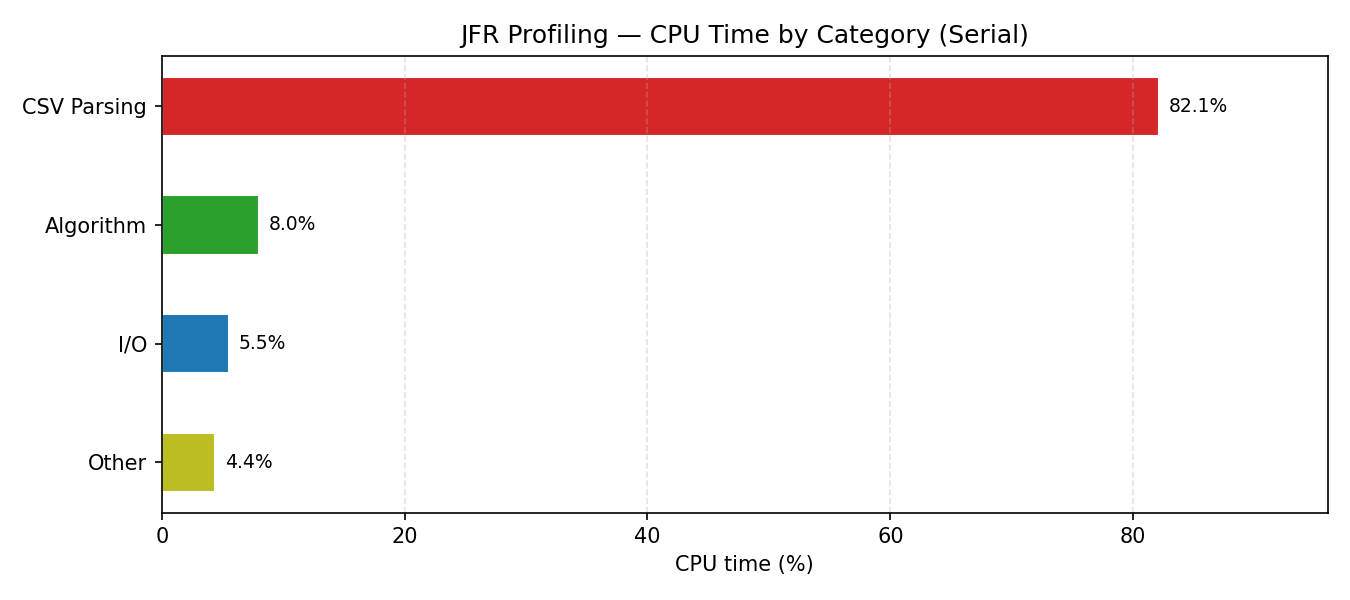
\includegraphics[width=0.82\textwidth]{img/chart4_jfr_hot_methods}
    \end{center}
    \vspace{-0.4em}
    {\small \alert{82\% do CPU} gasto convertendo texto para número --- o algoritmo em si representa apenas 8\%.}
\end{frame}

\begin{frame}{Resultados --- Serial}
    \begin{columns}
        \begin{column}{0.5\textwidth}
            \textbf{Microbenchmark (JMH)}
            \begin{itemize}
                \item Execução completa: \alert{212 s}
                \item Custo por iteração: \alert{$\approx$12 s}
                \item \texttt{closestCentroid}: 96 ns/chamada
                \item \texttt{squaredDistance}: 9 ns/chamada
            \end{itemize}
        \end{column}
        \begin{column}{0.5\textwidth}
            \textbf{Macrobenchmark (JMeter)}
            \begin{itemize}
                \item 1 thread: 1,56 exec/min
                \item 16 threads: 4,66 exec/min
                \item Ganho de $\approx$3$\times$ com 16$\times$ mais threads
                \item GC: $<$1\% do tempo total
            \end{itemize}
        \end{column}
    \end{columns}

    \vspace{0.6em}
    \begin{alertblock}{Diagnóstico}
        O gargalo não é a CPU --- é a conversão do CSV a cada iteração.
        Paralelizar a aritmética sozinha não vai ajudar.
    \end{alertblock}
\end{frame}

\begin{frame}{Comparação de Coletores de GC --- Throughput}
    Três coletores testados com 1, 2, 4, 8 e 16 threads JMeter (implementação serial):

    \vspace{0.8em}
    \begin{center}
    \begin{tabular}{lrr}
        \toprule
        \textbf{Coletor} & \textbf{1 thread} & \textbf{16 threads} \\
        \midrule
        G1GC (padrão JDK 25) & 1,56 exec/min & 4,66 exec/min \\
        ZGC                  & 1,50 exec/min & 4,40 exec/min \\
        ParallelGC           & 1,52 exec/min & \alert{4,85 exec/min} \\
        \bottomrule
    \end{tabular}
    \end{center}
\end{frame}

\begin{frame}{Comparação de Coletores de GC --- Conclusão}
    \begin{itemize}
        \item \textbf{ParallelGC} lidera levemente em alta carga --- otimizado para vazão
        \item \textbf{ZGC} fica um pouco atrás --- suas barreiras de escrita têm custo extra
        \item \textbf{G1GC} equilibrado, entre os dois
        \item Pausas de GC somam \alert{$<$1\%} do tempo em todos os casos
    \end{itemize}

    \vspace{1em}
    \begin{block}{O padrão se repete nas variantes v2}
        Coletor de GC não é o gargalo. A escolha tem impacto marginal no throughput.
    \end{block}
\end{frame}
